\graphicspath{{./figs/Chp-RelGaBP/}}


%%Fakesection Acronym reset
\glsreset{acr:rgabp}
\glsreset{acr:drgabp}
\glsreset{acr:sdd}
\glsreset{acr:wdd}


\chapter{Relaxed Gaussian Belief Propagation}
\label{chp:relGaBP}
%%Fakesection Abstract
The solution developed in this chapter is motivated by the fact that the \gls{acr:pwgabp} solver requires a large number of iterations to converge if the sparse matrix is \gls{acr:wdd} or is ill-conditioned.
Such matrices can arise from many application domains including the \gls{acr:fem}.
In this work, we present a relaxed form of \gls{acr:pwgabp} that reduces the number of iterations, resulting in significant computational reduction (up to 12.7$\times$) for ill-conditioned large linear systems.
In addition, to circumvent the need of determining the relaxation factor for the new algorithm a priori, we propose a second algorithm that incrementally determines a suitable relaxation factor based on iterative error improvements that also results in similar reductions in \gls{acr:pwgabp} iterations.
We show that the new algorithms can be implemented without any significant increase, over the original \gls{acr:pwgabp}, in both the computational complexity and the memory requirements.
We demonstrate the advantages of our algorithms using empirical results of large, ill-conditioned, and \gls{acr:wdd} matrices.


\section{Introduction}

\gls{acr:pwgabp} was empirically found to exhibit fast convergence for problems where the inverse covariance matrix of the underlying multivariate Gaussian distribution, or similarity the matrix $A$ of the sparse linear system, is \gls{acr:sdd} \cite{bib:Weiss01CorrectnessBelief, bib:Shental2008GBPSSLE}, especially when compared to the \gls{acr:dpcg} solver as shown in \chpRef{chp:PW-GaBP}.
However, if $A$ is large, sparse and ill-conditioned, then \gls{acr:pwgabp} may require a large number of iterations.
The work in \cite{bib:Weiss01CorrectnessBelief} provides a rough upper bound on the number of iterations required by \gls{acr:pwgabp} to reach a given convergence tolerance $\epsilon$; however, it is only applicable for \gls{acr:sdd} matrices.
The work in \cite{bib:Shental2008GBPSSLE} uses a common convergence acceleration method referred to as the Aitken-Steffensen's acceleration to speedup the \gls{acr:pwgabp} convergence.
In the Aitken-Steffensen's acceleration scheme, an improved estimate of a message is computed at each third iteration as:
\begin{equation}
	m\approx \hat{m}^{(t)}=m^{(t-3)}-\frac{(m^{(t-2)}-m^{(t-3)})^{2}}{m^{(t-1)}-2m^{(t-2)}+m^{(t-3)}}
\end{equation}
where $m^{(t)}$ represents a message estimate at iteration $t$. 
However, when this acceleration is used in \gls{acr:pwgabp} with ill-conditioned matrices, it yields unstable results even with double-precision implementations.
In addition, this acceleration scheme requires the additional storage of prior iteration messages which makes it very costly when implemented for large problems.


In this study, we will consider ill-conditioned matrices that are not necessarily \gls{acr:sdd}, which require considerably larger number of \gls{acr:pwgabp} iterations.
Finding a theoretical upper bound for the convergence rate of \gls{acr:pwgabp} for such matrices is still an open research question.
In addition, some of the solutions developed in this chapter are not only applicable to \glspl{acr:pwgm} but, rather, can also be used for general \glspl{acr:gm} such as the ones developed for the \gls{acr:fem} problem as will be illustrated in \chpRef{chp:FGaBP}.
However, since in this chapter the numerical analyses of the new solution were all performed in comparison with the original \gls{acr:pwgabp}, we will present the new formulation as an extension of the \gls{acr:pwgabp} solver.


This chapter is organized as follows.
In \secRef{sec:rgabp}, we present the new relaxation scheme for the \gls{acr:pwgabp} algorithm.
\secRef{sec:argabp} presents the dynamic relaxation algorithm.
Finally, in \secRef{sec:argabpResults} we present the numerical results and concluding remarks.


\section{The Relaxed PW-GaBP Algorithm}
\label{sec:rgabp}


In this section we will detail the relaxation formulation of the \gls{acr:pwgabp} algorithm, which was previously presented in the background chapter in \secRef{sec:pwgabp}.
We will proceed with our discussion whereby all the information available from the underlying problem is the matrix $A$.
In addition, we consider matrices that are large, sparse, ill-conditioned, and \gls{acr:wdd}.
With such matrices, the original \gls{acr:pwgabp} algorithm is known to require a very large number of iterations to converge.


\subsection{Edge Message Relaxation}


As can be seen from (\ref{eqn_a_i_minus_j_bc}), (\ref{eqn_b_i_minus_j_bc}) and (\ref{eqn_x_i}), the marginal mean of node $i$, which is also the solution estimate of $U_i^{(t)}$ at iteration $t$, can be obtained using the two sums $\alpha_i^{(t)}$ and $\beta_i^{(t)}$ of messages received on all connected edges $\mathcal{N}(i)$.
It can also be noted from these equations that applying any relaxation on the $\beta$ messages does not affect the $\alpha$ messages convergence properties.  Relaxation on $\beta_{ij}$ can be applied as follows:
\begin{equation}
	\hat{\beta}_{ij}^{(t)} = \gamma \beta_{ij}^{(t)} + (1-\gamma)\beta_{ij}^{(t-1)}
\end{equation}
where $\gamma$ is referred to as the relaxation factor.
The relaxation factor $\gamma$ is obtained from the limit  $\gamma \in [0,2]$.
If $\gamma$ is in $[0,1]$, the method is referred to as under-relaxation or damping and, in certain cases, is used to force a divergent \gls{acr:pwgabp} to converge at the expense of a high iteration count.
If $\gamma $ is in $[1,2]$, the method is referred to as over-relaxation and is used to accelerate convergence, which is the objective of this work.  
The new relaxed message $\hat{\beta}_{ij}^{(t)}$ can be communicated instead of $\beta_{ij}^{(t)}$.
It can be seen that if $\gamma$ is chosen such that the \gls{acr:pwgabp} algorithm is convergent, the relaxed messages converge as $\beta_{ij}^{(t)} \approx \beta_{ij}^{(t-1)}$.
This indicates that the stationarity point of the relaxed algorithm is that of the original \gls{acr:pwgabp}.
We refer to this style of relaxation as \gls{acr:emr}.
It is clear that this relaxation does not require additional memory since it only requires the previous iteration message.
The \gls{acr:emr} relaxation is the most flexible and can be applied to any \gls{acr:gm}.


\subsection{Nodal Message Relaxation}


An alternative strategy to \gls{acr:emr}, we can apply relaxation to the nodal sum $\beta_i$ messages as opposed to each individual edge message $\beta_{ij}$.
The $\beta_i$ messages are then relaxed as follows:
\begin{equation}
	\hat{\beta}_{i}^{(t)} = \gamma \beta_{i}^{(t)} + (1-\gamma)\beta_{i}^{(t-1)} \label{eq_relx_b_i}.
\end{equation}
We refer to this relaxation scheme as the \gls{acr:nmr}.
Relaxing $\beta_i$ messages requires additional memory of order $\bigo{N}$ to store the previous iteration's $\beta_{i}^{(t-1)}$ value.
However, based on the distinct observation that for every matrix we tested from the class of \gls{acr:wdd} matrices, the $\alpha$ messages converged much faster than the $\beta$ messages to within 10 to 20 iterations as demonstrated by our empirical results.
If we decide to use this property, we can eliminate the additional memory requirement due to relaxing $\beta_i$ messages by reformulating the updates as follows: 
\begin{align}
	\hat{\beta}_{i}^{(t+t_{o})} & =  \alpha_{i}^{*}\hat{\mu}_{i}^{(t+t_{o})}  \\
	\intertext{where:}
	\hat{\mu}_{i}^{(t+t_{o})} & =  \gamma \mu_{i}^{(t+t_{o})}+(1-\gamma)\mu_{i}^{(t+t_{o}-1)} \label{eq_relx_x_i}
\end{align}
where $\alpha_i^*$ is the fixed point reached after $t_o$ iterations.
The $\mu_{i}^{(t-1)}$ values are reused here since they are used to store the final solution.

To illustrate the correctness of the \gls{acr:nmr} based on the original \gls{acr:pwgabp} update rules of $\beta_{ij}$ messages, we substitute (\ref{eq_relx_b_i}) into (\ref{eqn_b_i_minus_j_bc}) and then into (\ref{eqn_GaBPUpdateM}) to obtain the following:
\begin{align}
	\hat{\beta}_{ij}^{(t+t_{o})} & = \frac{-A_{ij}}{\alpha_{i\setminus j}^{*}}\hat{\beta}_{i\setminus j}^{(t+t_{o})}\\
	\intertext{where,}
	\hat{\beta}_{i\setminus j}^{(t+t_{o})} & = \hat{\beta}_{i}^{(t+t_{o})}-\beta_{ji}^{(t+t_{o})}\\ 
	\begin{split}
		& = \gamma\beta_{i\setminus j}^{(t+t_{o})}+(1-\gamma)\beta_{i\setminus j}^{(t+t_{o}-1)} \\  
		& \quad -(1-\gamma)\Delta\beta_{ji}^{(t+t_{o})}
	\end{split}
	\intertext{and,}
	\Delta\beta_{ji}^{(t+t_{o})} &= \beta_{ji}^{(t+t_{o})} - \beta_{ji}^{(t+t_{o}-1)}.
\end{align}
It can be seen from the above modified \gls{acr:bp} rule for $\beta_{ij}$ messages that if $\gamma$ is chosen such that the relaxed \gls{acr:pwgabp} is convergent, the additional terms $ \Delta\beta_{ji}^{(t+t_{o})}, \forall j $ will approach zero and the relaxed algorithm's fixed point will be equal to the fixed point solution of the original \gls{acr:pwgabp} algorithm.
The listing of the relaxed \gls{acr:pwgabp} algorithm is shown in \algRef{alg:relaxed_gabp}. 
We refer to this algorithm as the \gls{acr:rgabp} algorithm.

\begin{algorithm}[h]
	\centering
	\begin{algorithmic}[1]
		\STATE \textit{Initialize: $\forall i,j$}\\
%\setlength{\belowdisplayskip}{0pt}
%\setlength{\abovedisplayskip}{0pt}
%\begin{align*}
		\begin{tabular}{cc}
			$\alpha_{ij} = 0$ & $ \beta_{ij} = 0$\\ 
			$\gamma \in [1,2]$ & $u_i^{(0)} = 0$
		\end{tabular}
%\end{align*}
		\REPEAT[Start \gls{acr:pwgabp} iteration: $t=1,2,\cdots$]
		\FOR{ each node $i$ }
		\STATE $\alpha_{i} = A_{ii} + \sum_{k \in N(i)} \alpha_{ki}$
		\STATE $\beta_{i} = b_{i} + \sum_{k \in N(i)} \beta_{ki}$
		\IF{$ \frac{\parallel \Delta\alpha_i \parallel}{\parallel \alpha \parallel} < \epsilon\; \forall i$}\label{test}
		\STATE $\hat\beta_i = \gamma\beta_i + (1-\gamma)\alpha_i \mu_i^{(t-1)}$ \COMMENT{Relaxation using $\gamma$} 
		\ELSE
		\STATE $\hat\beta_i = \beta_i$ 
		\AlgENDIF
		\STATE $\mu_i = \hat{\beta}_i / \alpha_i$
		\STATE \COMMENT{Message update subject to a schedule}
		\FOR{ each edge $i \rightarrow j$ } 
		\STATE $\alpha_{ij} = -A_{ij}^2 (\alpha_{i}-\alpha_{ji})^{-1} $
		\STATE $\beta_{ij} = -A_{ij} ( \hat\beta_{i}-\beta_{ji})(\alpha_{i}-\alpha_{ji})^{-1} $
		\AlgENDFOR
		\AlgENDFOR
		\STATE Compute:  $e_r = \left(\frac{\sum (\mu_i - \mu_i^{(t-1)})^2} {\sum \mu_i^2} \right)^{\frac{1}{2}}$
		\UNTIL{Convergence check: $e_r < \epsilon$ }
		\STATE \textit{Output:} $\overline{u} = \left[ \mu_i \right] \forall i$
	\end{algorithmic}
	\caption{The \acrshort{acr:rgabp} algorithm.}
	\label{alg:relaxed_gabp}
\end{algorithm}

The condition for variance convergence in step-\ref{test} of \algRef{alg:relaxed_gabp} is not inherently required but rather is used to reduce the memory requirement.
As explained earlier, once the variances converge, we can obtain $ \beta_i^{(t-1)}$ from $u_i^{(t-1)}$ in order to relax $\beta_i^{(t)}$ which saves implementation memory of up to $O \left( N \right)$.  

By using an over-relaxation factor $\gamma \in [1,2]$, our empirical results indicate that the optimal $\gamma_\mathit{opt}$ that yields the lowest iteration count for a given tolerance ($\epsilon$) for the relative norm, as defined in \secRef{sec:convtest}, depends strongly on the elements of the matrix $A$, which makes $\gamma_\mathit{opt}$ dependent on the underlying problem.
Hence, finding a suitable $\gamma$ may prove difficult especially since using the wrong value will cause the algorithm to fail to converge.
In the following section, we propose a heuristic algorithm that iteratively and incrementally finds an approximation to $\gamma$ that, in general, produces a sufficiently fast convergence by iteratively reducing the relative norm.


\section{Dynamic Over-relaxation}
\label{sec:argabp}

The solution presented here, which circumvents determining $\gamma_{opt}$ a priori, is motivated by the following empirical observations of the \gls{acr:rgabp} algorithm: a threshold $\gamma_\mathit{opt}$ exists in the interval $[1,2]$ that is also found to be a maximum in the same interval for given initial conditions, any further increase in $\gamma_{opt}$ will cause a substantial increase in $ e_r^{(t)}$.
As a result, we can propose a dynamic update scheme for $\gamma$ based on the progress of the \gls{acr:rgabp} relative norm.
More precisely, we can gradually increase $\gamma$ starting from an initial value by adding an increment $\Delta\gamma$ each $d$ number of iterations as long as the $e_r$ is improving.
However, if $e_r$ is found not to improve, we can likewise decrement $\gamma$.
\algRef{alg:gamma_update} shows the details of an algorithm that can be used to find a rough estimate of the over-relaxation $\gamma$ which results in a high relative norm decrease rate. 


\begin{algorithm}[h]
	\centering
	\begin{algorithmic}[1]
		\STATE \textit{Initialize:}\\
		\begin{tabular}{ll}
			$e_\mathit{best} = 1.0$ & $\gamma^{(0)}  = 1.0$\\ 
			$d  = 10$ & $\Delta\gamma  = 0.1$
		\end{tabular}
		\REPEAT[\gls{acr:pwgabp} iteration: $t=1,2,\cdots$]
		\IF{$ t\mod{d} = 0$}
		\IF{$e_r^{(t)} < e_\mathit{best}$}
		\STATE $\gamma^{(t)} = \gamma^{(t-1)} + \Delta\gamma$ \COMMENT {Increment $\gamma$}
		\STATE $e_\mathit{best} = e_r^{(t)}$
		\ELSE
		\STATE $\gamma^{(t)} = \gamma^{(t-1)} - \Delta\gamma$ \COMMENT{Decrement $\gamma$}
		\IF{$\gamma^{(t)} < 1.0$}
		\STATE $\gamma^{(t)} = 1.0$
	\ENDIF
\ENDIF
\ENDIF
\UNTIL{\gls{acr:pwgabp} terminates }
\end{algorithmic}
\caption{The \gls{acr:drgabp} algorithm.}
\label{alg:gamma_update}
\end{algorithm}


\algRef{alg:gamma_update} relies on two basic settings $\Delta \gamma$ and $d$.
The parameter $\Delta \gamma$ is a fixed increment or decrement size which nominally can be set to $0.1$, while $d$ is the iteration interval length on which $e_r$ can be tested in order to adjust $\gamma$.
The relative norm sampling interval $d$ should be chosen wide enough so that the fluctuations in $e_r$, resulting from the prior $\gamma$ change, can diminish resulting in a stable value for $e_r$ that can be sampled.
In all of the cases we analyzed for ill-conditioned \gls{acr:wdd} matrices, a good value for $d$ was found to be around 10 to 20 iterations.
We refer to this algorithm as the \gls{acr:drgabp} algorithm.


If $\Delta\gamma$ is chosen sufficiently small with a sufficiently wide relative norm sampling iteration interval $d$, the \gls{acr:drgabp} algorithm should converge.
Unlike the Aitken-Steffensen or similar acceleration methods, this algorithm is computationally more stable specially for ill-conditioned matrices.
Another key advantage of the \gls{acr:drgabp} algorithm is that it does not require a significant increase in both computation and memory over the original \gls{acr:pwgabp} algorithm. 


\section{Results and Discussions}
\label{sec:argabpResults}

The test matrices are obtained from the classical L-shaped conductor problem in electromagnetics.
As shown in \figRef{fig:L-shaped}, the potential in the space between the two square conductors carrying different voltages is found by solving the Laplace equation, $ \nabla^2 u = 0 $.
However in practice, Laplace's equation is solved numerically by the \gls{acr:fem}, which starts by dividing the interconductor space into triangular elements.
Using a first order \gls{acr:fem},  the problem typically requires the solution of a linear system of equations that is large, sparse, ill-conditioned, and \gls{acr:wdd}.
In this section, we demonstrate the effectiveness of our developed algorithms, the \gls{acr:rgabp} and the \gls{acr:drgabp}, by solving the linear system arising from this Laplace problem.
We also use a selected set of other generated matrices in order to illustrate our empirical results.
We used asynchronous message scheduling for all our algorithms.
The relative norm $e_r$ is recorded at each iteration.
All algorithms were terminated when the normalized residual ($l^2$-norm) reached $R < 10^{-9}$.

\begin{figure}[h]
	\centerline{
	\subfloat[]{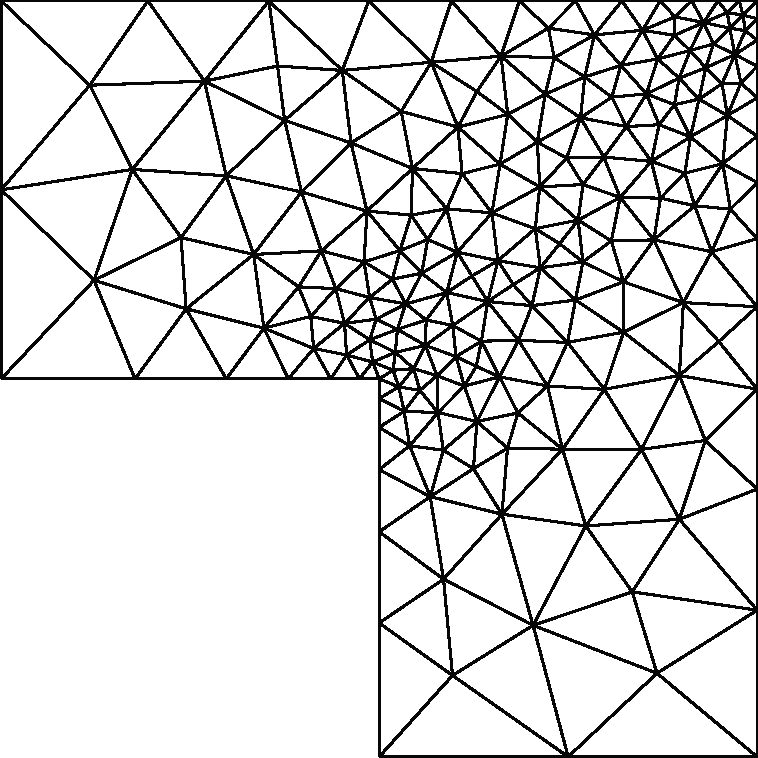
\includegraphics[width=1.75in]{L-shaped}}
	\hspace{2em}
	\subfloat[]{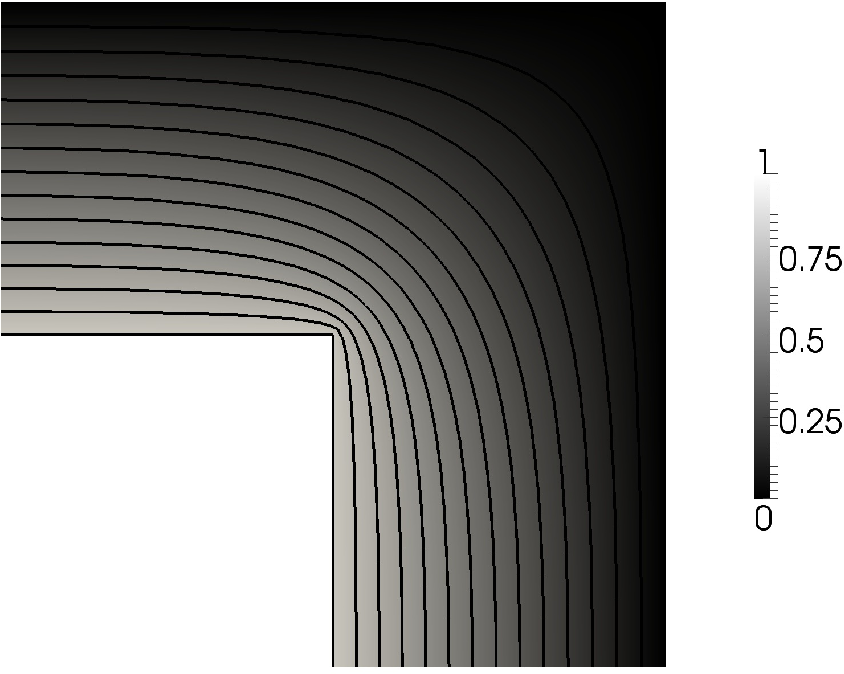
\includegraphics[width=2.2in]{L-shaped_sol}}
	}
	\caption[The L-shaped conductor problem.]{L-shaped conductor problem of dimensions equal to 1cm. (a) Illustrated discretization using a small mesh. (b) Equipotential lines of the potential solution of the Laplace's equation, volts scale.}
	\label{fig:L-shaped}
\end{figure}

The plots in \figRef{fig:err_rlx} demonstrate the iteration reduction due to the \gls{acr:rgabp} algorithm.
The  size of the linear system characterized by the matrix $A$ is $N=2700$ unknowns, with number of non-zeros $\gls{acr:nnz} = 17572$.
The original \gls{acr:pwgabp} algorithm required 2449 iterations while the \gls{acr:rgabp} algorithm required as low as 389 iterations for $\gamma = 1.538$ resulting in a reduction factor of 6.2.
It can be observed that the overall relative norm decreases consistently as $\gamma$ increases to a certain value in the interval $[1,2]$.
It is expected that for this problem the best $\gamma_\mathit{opt}$ can be empirically obtained as $\gamma_\mathit{opt} \approx 1.538$, any further increase on $\gamma$ will cause $e_r$ to increase, and consequently causing the algorithm to fail to converge.


\begin{figure}[h]
	\centering
	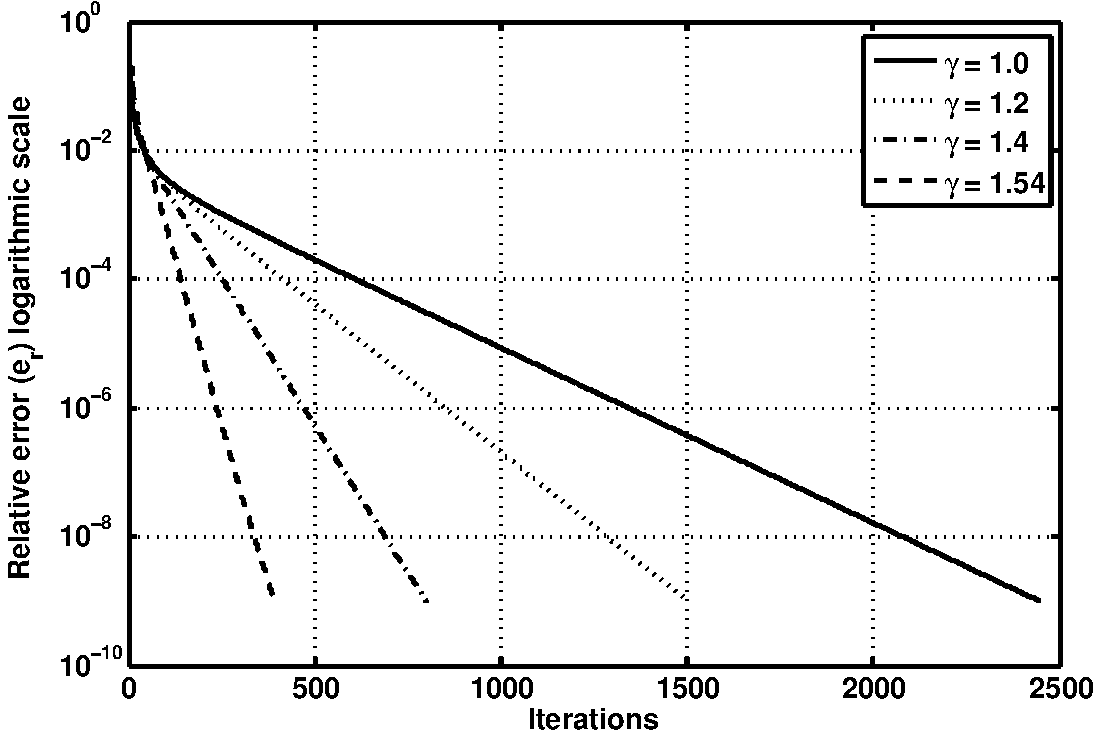
\includegraphics[width=4in]{err_plot_1}
	\caption[Performance of the \acrshort{acr:rgabp} for different relaxation factors.]{The relative norm $e_r$ plots for the \gls{acr:rgabp} algorithm with different relaxation factors $\gamma$.}
	\label{fig:err_rlx}
\end{figure}

The plots in \figRef{fig:err_IncRlx} show the results of the \gls{acr:drgabp} algorithm in obtaining a considerably lower \gls{acr:pwgabp} iteration count without prior knowledge of $\gamma_{opt}$.
The parameter $\Delta\gamma$ is varied from the fine value of $10^{-2}$ to the coarser value of $2\times 10^{-1}$.
A relative norm sampling interval of $d = 10$ was used for all plots.
It is worth noting here that the best iteration reduction was found for $\Delta\gamma = 2\times 10^{-1}$ resulting in 337 iterations.
This is lower than the previously reported 389 iterations by \gls{acr:rgabp} assuming prior knowledge of $\gamma_{opt}$.
This reduction may be attributed to the dynamics of the algorithm in alternating between two values of $\gamma$ which are (1.3 and 1.6). 

\begin{figure}[h]
	\centering
	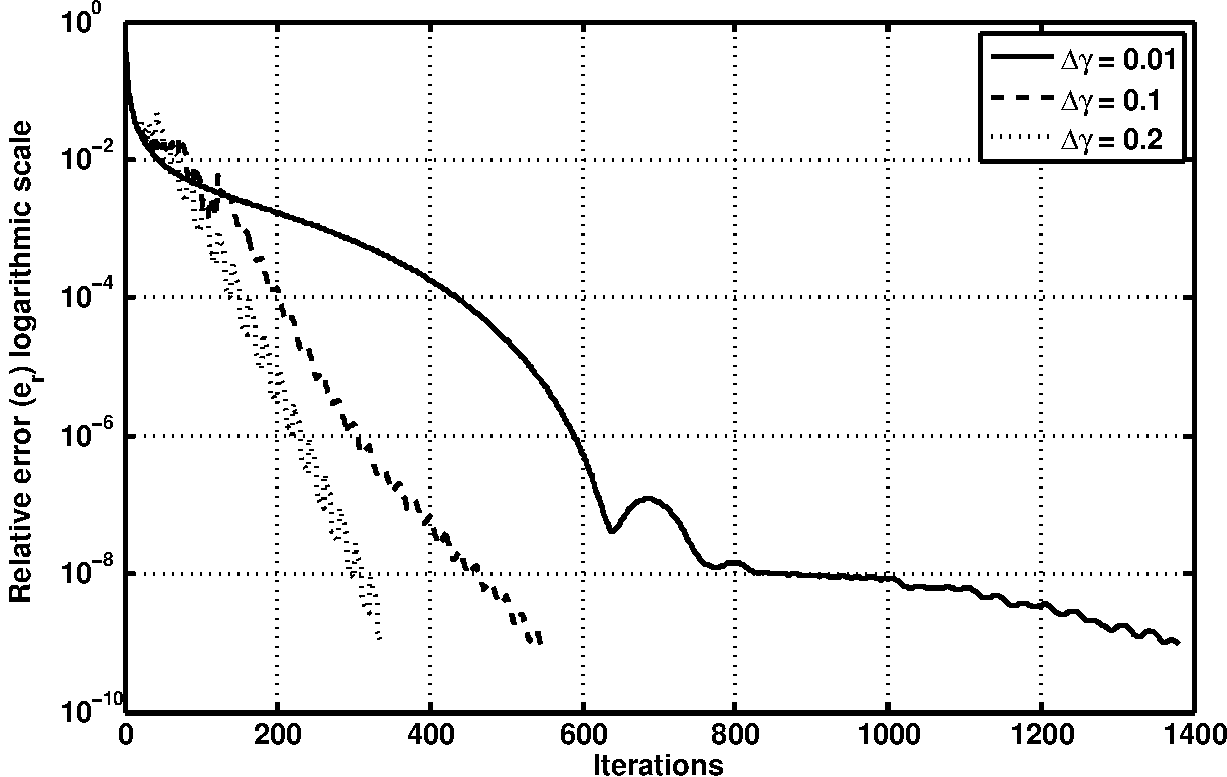
\includegraphics[width=4in]{err_plot_2}
	\caption[Performance of \acrshort{acr:drgabp} for different relaxation increments.]{The relative norm $e_r$ plots for the \gls{acr:drgabp} algorithm with different relaxation increments $\Delta\gamma$.}
	\label{fig:err_IncRlx}
\end{figure}

The case of \gls{acr:drgabp} with $\Delta\gamma = 10^{-2}$ resulted in 1381 iterations.
While this performance is still considerably better than the original \gls{acr:pwgabp}, the larger comparative iterations may be attributed to the fact that $\gamma$ fluctuates between two values which do not necessarily produce the lowest overall relative norm.
However, the algorithm converged for all considered values of $\Delta\gamma$.
In general, the smaller the values of $\Delta\gamma$ are, the wider the applicability of the algorithm at the expense of a higher iteration count.
We found that the nominal $\Delta\gamma = 10^{-1}$ is suitable for most matrices that are ill-conditioned and weakly diagonally dominant.   


We illustrate in \tableRef{tbl:testmatrices_RGaBP} a selected set of test matrices.
One matrix was obtained from the Matrix Market website repository \cite{bib:matrixMarket}.
The other two matrices were generated randomly using Matlab and set to be sparse and \gls{acr:wdd}.
The generated matrices all have negative off-diagonals which results in ill-conditioned matrices.
For all algorithms we used $d = 10$.
The variances for all matrices converged in less than 10 iterations.
The density \% of the matrix is measured by $\gls{acr:nnz} / N^2 \times 100$.

\tableRef{tbl:testmatrices_RGaBP} demonstrates that reductions in iterations were produced by the \gls{acr:rgabp} algorithm in all test cases.
The second matrix shows a reduction factor of 12.7 for $ \gamma = 1.8 $.
\tableRef{tbl:testmatrices_DRGaBP} shows the results of \gls{acr:drgabp} which also produced significant iteration reductions versus the original \gls{acr:pwgabp}.
The performance of \gls{acr:drgabp} algorithm can depend on the choice of $\Delta\gamma$, however the algorithm converged in all tested cases.
It was observed that the nominal value of $\Delta\gamma = 0.1$ resulted in best reductions on average.

\begin{table}[h]
	\centering
	\begin{threeparttable}[c]
		\caption{Results for the \acrshort{acr:rgabp} algorithm on selected test matrices.}
		\label{tbl:testmatrices_RGaBP}
		\begin{tabular}{ccccccc}
			\toprule
			\multirow{2}{*}{Matrix} & \multirow{2}{*}{N} & Density & \multirow{2}{*}{\gls{acr:pwgabp}} & \multicolumn{2}{c}{R-GaB} & Red.\tabularnewline
			\cline{5-6} 
			&  & (\%) &  & Itrs & $\gamma$ & Factor\tabularnewline
			\midrule 
			gr\_30\_30 \cite{bib:matrixMarket} & 900 & 0.956 & 859 & 115 & 1.59 & 7.5\tabularnewline
			Sp Rand 1 & 5000 & 0.4 & 5571 & 437 & 1.8 & 12.7\tabularnewline
			Sp Rand 2 & 3000 & 0.4 & 3028 & 241 & 1.67 & 12.6\tabularnewline
			\bottomrule
		\end{tabular}
	\end{threeparttable}
\end{table}


\begin{table}[h]
	\centering
	\begin{threeparttable}[c]
		\caption{Results for the \acrshort{acr:drgabp} algorithm on selected test matrices.}
		\label{tbl:testmatrices_DRGaBP}
		\centering
		\begin{tabular}{ccccc}
			\toprule
			\multirow{2}{*}{Matrix} & \multicolumn{3}{c}{\gls{acr:drgabp}} & Red. Factor\tabularnewline
			\cline{2-4} 
			& $\Delta\gamma=0.01$ & $\Delta\gamma=0.1$ & $\Delta\gamma=0.2$ & $\Delta\gamma=0.1$\tabularnewline
			\midrule 
			gr\_30\_30 \cite{bib:matrixMarket} & 456 & 783 & 647 & 1.1\tabularnewline
			Sp Rand 1 & 1873 & 872 & 1492 & 6.4\tabularnewline
			Sp Rand 2 & 732 & 759 & 963 & 4.0\tabularnewline
			\bottomrule
		\end{tabular}
	\end{threeparttable}
\end{table}


\section{Conclusion}
We have presented the \gls{acr:rgabp} algorithm which implements new relaxation schemes for the \gls{acr:pwgabp} algorithm to considerably accelerate its convergence for ill-conditioned \gls{acr:wdd} inverse covariance matrices.
We have demonstrated empirical reductions in iterations of up to 12.7 times.
We have also introduced the \gls{acr:drgabp} algorithm that avoids the complexity of setting a prior over-relaxation factor.
The \gls{acr:drgabp} algorithm demonstrates performance comparable with the \gls{acr:rgabp} algorithm with a prior knowledge of an optimal relaxation factor.
The new algorithms do not require any increase of the computational complexity or the memory requirements of the original \gls{acr:pwgabp} algorithm hence facilitating efficient implementations on parallel architectures.


